\coverchapter{Connections created by bijections}\label{ch:connect}

% experimental class 1
\begin{figure}[ht!]
    \centering
    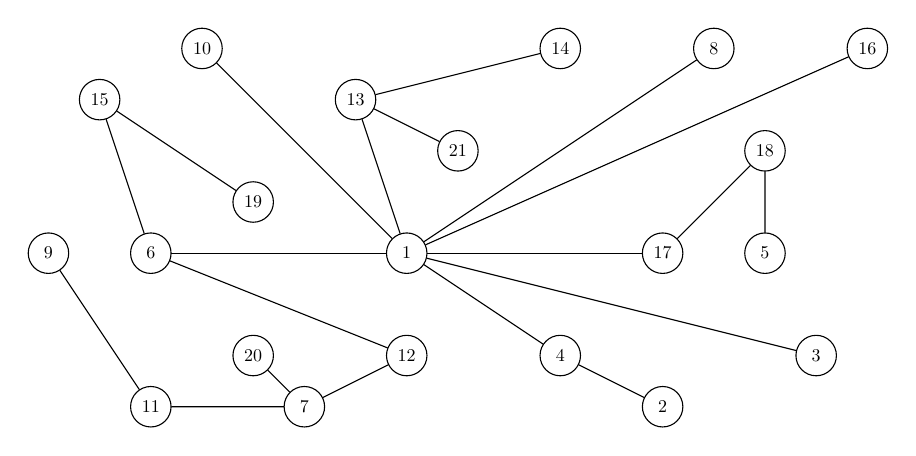
\begin{tikzpicture}[vertex/.style = {shape=circle,draw,minimum size=2.25em},scale=0.65, every node/.style={scale=0.65}]
\node[vertex] (c1) at (0,0) {$1$};
\node[vertex] (c2) at (5,-3) {$2$};
\node[vertex] (c3) at (8,-2) {$3$};
\node[vertex] (c4) at (3,-2) {$4$};
\node[vertex] (c5) at (7,0) {$5$};
\node[vertex] (c6) at (-5,0) {$6$};
\node[vertex] (c7) at (-2,-3) {$7$};
\node[vertex] (c8) at (6,4) {$8$};
\node[vertex] (c9) at (-7,0) {$9$};
\node[vertex] (c10) at (-4,4) {$10$};
\node[vertex] (c11) at (-5,-3) {$11$};
\node[vertex] (c12) at (0,-2) {$12$};
\node[vertex] (c13) at (-1,3) {$13$};
\node[vertex] (c14) at (3,4) {$14$};
\node[vertex] (c15) at (-6,3) {$15$};
\node[vertex] (c16) at (9,4) {$16$};
\node[vertex] (c17) at (5,0) {$17$};
\node[vertex] (c18) at (7,2) {$18$};
\node[vertex] (c19) at (-3,1) {$19$};
\node[vertex] (c20) at (-3,-2) {$20$};
\node[vertex] (c21) at (1,2) {$21$};
\draw (c1) -- (c4);
\draw (c1) -- (c6);
\draw (c1) -- (c8);
\draw (c1) -- (c13);
\draw (c1) -- (c16);
\draw (c1) -- (c17);
\draw (c2) -- (c4);
\draw (c5) -- (c18);
\draw (c6) -- (c12);
\draw (c6) -- (c15);
\draw (c7) -- (c11);
\draw (c7) -- (c12);
\draw (c7) -- (c20);
\draw (c9) -- (c11);
\draw (c13) -- (c14);
\draw (c13) -- (c21);
\draw (c15) -- (c19);
\draw (c17) -- (c18);
\draw (c1) -- (c3);
\draw (c1) -- (c10);
\end{tikzpicture}
    \caption{The connections created by bijections for experimental class I.}
    \label{fig:expgrp_I}
\end{figure}


% experimental class 2
\begin{figure}[ht!]
    \centering
    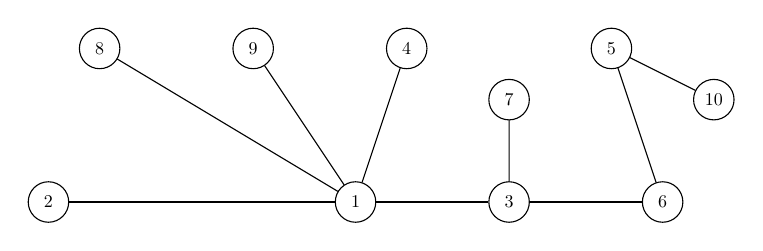
\begin{tikzpicture}[vertex/.style = {shape=circle,draw,minimum size=2.25em},scale=0.65, every node/.style={scale=0.65}]
    \node[vertex] (c1) at (0,0) {$1$};
    \node[vertex] (c2) at (-6,0) {$2$};
    \node[vertex] (c3) at (3,0) {$3$};
    \node[vertex] (c4) at (1,3) {$4$};
    \node[vertex] (c5) at (5,3) {$5$};
    \node[vertex] (c6) at (6,0) {$6$};
    \node[vertex] (c7) at (3,2) {$7$};
    \node[vertex] (c8) at (-5,3) {$8$};
    \node[vertex] (c9) at (-2,3) {$9$};
    \node[vertex] (c10) at (7,2) {$10$};
    \draw (c1) -- (c2);
    \draw (c1) -- (c3);
    \draw (c1) -- (c4);
    \draw (c1) -- (c8);
    \draw (c1) -- (c9);
    \draw (c3) -- (c6);
    \draw (c3) -- (c7);
    \draw (c5) -- (c6);
    \draw (c5) -- (c10);
\end{tikzpicture}
    \caption{The connections created by bijections for experimental class II.}
    \label{fig:expgrp_II}
\end{figure}


% experimental class 3
\begin{figure}[ht!]
    \centering
    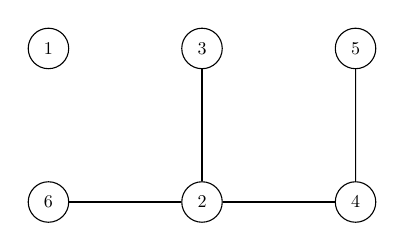
\begin{tikzpicture}[vertex/.style = {shape=circle,draw,minimum size=2.25em},scale=0.65, every node/.style={scale=0.65}]
    \node[vertex] (c1) at (-3,3) {$1$};
    \node[vertex] (c2) at (0,0) {$2$};
    \node[vertex] (c3) at (0,3) {$3$};
    \node[vertex] (c4) at (3,0) {$4$};
    \node[vertex] (c5) at (3,3) {$5$};
    \node[vertex] (c6) at (-3,0) {$6$};
    \draw (c2) -- (c3);
    \draw (c2) -- (c4);
    \draw (c2) -- (c6);
    \draw (c4) -- (c5);
\end{tikzpicture}
    \caption{The connections created by bijections for experimental class III where we failed to connect one permutation class.}
    \label{fig:expgrp_III}
\end{figure}


% experimental class 4
\begin{figure}[ht!]
    \centering
    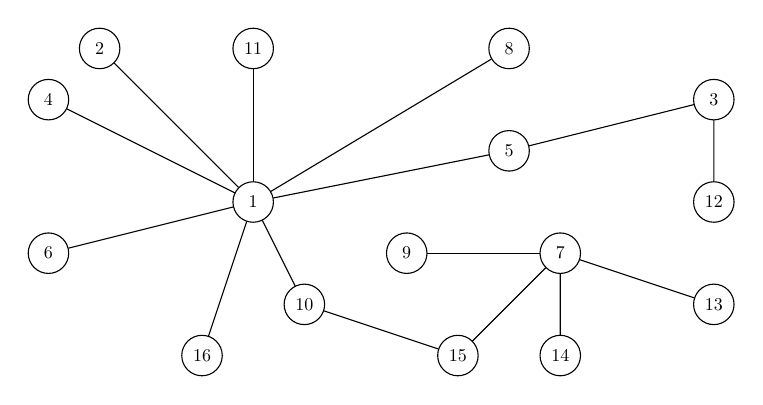
\begin{tikzpicture}[vertex/.style = {shape=circle,draw,minimum size=2.25em},scale=0.65, every node/.style={scale=0.65}]
    \node[vertex] (c1) at (0,0) {$1$};
    \node[vertex] (c2) at (-3,3) {$2$};
    \node[vertex] (c3) at (9,2) {$3$};
    \node[vertex] (c4) at (-4,2) {$4$};
    \node[vertex] (c5) at (5,1) {$5$};
    \node[vertex] (c6) at (-4,-1) {$6$};
    \node[vertex] (c7) at (6,-1) {$7$};
    \node[vertex] (c8) at (5,3) {$8$};
    \node[vertex] (c9) at (3,-1) {$9$};
    \node[vertex] (c10) at (1,-2) {$10$};
    \node[vertex] (c11) at (0,3) {$11$};
    \node[vertex] (c12) at (9,0) {$12$};
    \node[vertex] (c13) at (9,-2) {$13$};
    \node[vertex] (c14) at (6,-3) {$14$};
    \node[vertex] (c15) at (4,-3) {$15$};
    \node[vertex] (c16) at (-1,-3) {$16$};
    \draw (c1) -- (c2);
    \draw (c1) -- (c4);
    \draw (c1) -- (c5);
    \draw (c1) -- (c10);
    \draw (c1) -- (c11);
    \draw (c1) -- (c16);
    \draw (c3) -- (c12);
    \draw (c7) -- (c9);
    \draw (c7) -- (c13);
    \draw (c7) -- (c14);
    \draw (c7) -- (c15);
    \draw (c10) -- (c15);
    \draw (c1) -- (c6);
    \draw (c1) -- (c8);
    \draw (c3) -- (c5);
\end{tikzpicture}
    \caption{The connections created by bijections for experimental class IV.}
    \label{fig:expgrp_IV}
\end{figure}


% experimental class 5
\begin{figure}[ht!]
    \centering
    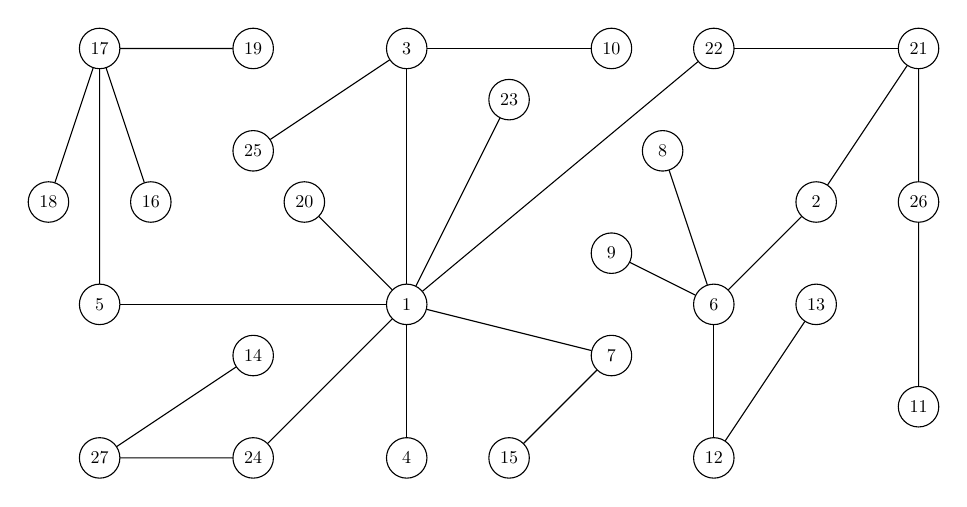
\begin{tikzpicture}[vertex/.style = {shape=circle,draw,minimum size=2.25em},scale=0.65, every node/.style={scale=0.65}]
    \node[vertex] (c1) at (0,0) {$1$};
    \node[vertex] (c2) at (8,2) {$2$};
    \node[vertex] (c3) at (0,5) {$3$};
    \node[vertex] (c4) at (0,-3) {$4$};
    \node[vertex] (c5) at (-6,0) {$5$};
    \node[vertex] (c6) at (6,0) {$6$};
    \node[vertex] (c7) at (4,-1) {$7$};
    \node[vertex] (c8) at (5,3) {$8$};
    \node[vertex] (c9) at (4,1) {$9$};
    \node[vertex] (c10) at (4,5) {$10$};
    \node[vertex] (c11) at (10,-2) {$11$};
    \node[vertex] (c12) at (6,-3) {$12$};
    \node[vertex] (c13) at (8,0) {$13$};
    \node[vertex] (c14) at (-3,-1) {$14$};
    \node[vertex] (c15) at (2,-3) {$15$};
    \node[vertex] (c16) at (-5,2) {$16$};
    \node[vertex] (c17) at (-6,5) {$17$};
    \node[vertex] (c18) at (-7,2) {$18$};
    \node[vertex] (c19) at (-3,5) {$19$};
    \node[vertex] (c20) at (-2,2) {$20$};
    \node[vertex] (c21) at (10,5) {$21$};
    \node[vertex] (c22) at (6,5) {$22$};
    \node[vertex] (c23) at (2,4) {$23$};
    \node[vertex] (c24) at (-3,-3) {$24$};
    \node[vertex] (c25) at (-3,3) {$25$};
    \node[vertex] (c26) at (10,2) {$26$};
    \node[vertex] (c27) at (-6,-3) {$27$};
    \draw (c1) -- (c3);
    \draw (c1) -- (c4);
    \draw (c1) -- (c7);
    \draw (c1) -- (c20);
    \draw (c1) -- (c22);
    \draw (c1) -- (c23);
    \draw (c1) -- (c24);
    \draw (c2) -- (c21);
    \draw (c3) -- (c10);
    \draw (c3) -- (c25);
    \draw (c6) -- (c9);
    \draw (c6) -- (c12);
    \draw (c11) -- (c26);
    \draw (c12) -- (c13);
    \draw (c14) -- (c27);
    \draw (c17) -- (c18);
    \draw (c17) -- (c19);
    \draw (c21) -- (c22);
    \draw (c21) -- (c26);
    \draw (c24) -- (c27);
    \draw (c1) -- (c5);
    \draw (c2) -- (c6);
    \draw (c5) -- (c17);
    \draw (c6) -- (c8);
    \draw (c7) -- (c15);
    \draw (c16) -- (c17);
\end{tikzpicture}
    \caption{The connections created by bijections for experimental class V.}
    \label{fig:expgrp_V}
\end{figure}


% experimental class 6 - Only 2 classes, no need to display
\begin{comment}
\begin{figure}[ht!]
    \centering
    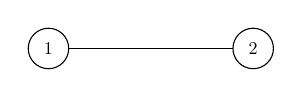
\begin{tikzpicture}[vertex/.style = {shape=circle,draw,minimum size=2.25em},scale=0.65, every node/.style={scale=0.65}]
    \node[vertex] (c1) at (0,0) {$1$};
    \node[vertex] (c2) at (4,0) {$2$};
    \draw (c1) -- (c2);
\end{tikzpicture}
    \caption{The connections created by bijections for experimental class VI.}
    \label{fig:expgrp_VI}
\end{figure}
\end{comment}


% experimental class 7 - Only 2 classes, no need to display
\begin{comment}
\begin{figure}[ht!]
    \centering
    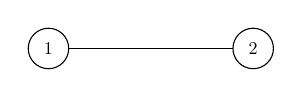
\begin{tikzpicture}[vertex/.style = {shape=circle,draw,minimum size=2.25em},scale=0.65, every node/.style={scale=0.65}]
    \node[vertex] (c1) at (0,0) {$1$};
    \node[vertex] (c2) at (4,0) {$2$};
    \draw (c1) -- (c2);
\end{tikzpicture}
    \caption{The connections created by bijections for experimental class VII.}
    \label{fig:expgrp_VII}
\end{figure}
\end{comment}


% experimental class 8 - Only 2 classes, no need to display
\begin{comment}
\begin{figure}[ht!]
    \centering
    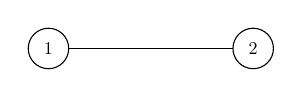
\begin{tikzpicture}[vertex/.style = {shape=circle,draw,minimum size=2.25em},scale=0.65, every node/.style={scale=0.65}]
    \node[vertex] (c1) at (0,0) {$1$};
    \node[vertex] (c2) at (4,0) {$2$};
    \draw (c1) -- (c2);
\end{tikzpicture}
    \caption{The connections created by bijections for experimental class VIII.}
    \label{fig:expgrp_VIII}
\end{figure}
\end{comment}


% experimental class 9
\begin{figure}[ht!]
    \centering
    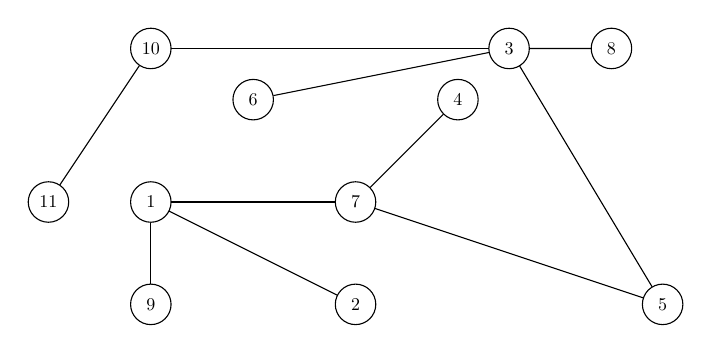
\begin{tikzpicture}[vertex/.style = {shape=circle,draw,minimum size=2.25em},scale=0.65, every node/.style={scale=0.65}]
    \node[vertex] (c1) at (0,0) {$1$};
    \node[vertex] (c2) at (4,-2) {$2$};
    \node[vertex] (c3) at (7,3) {$3$};
    \node[vertex] (c4) at (6,2) {$4$};
    \node[vertex] (c5) at (10,-2) {$5$};
    \node[vertex] (c6) at (2,2) {$6$};
    \node[vertex] (c7) at (4,0) {$7$};
    \node[vertex] (c8) at (9,3) {$8$};
    \node[vertex] (c9) at (0,-2) {$9$};
    \node[vertex] (c10) at (0,3) {$10$};
    \node[vertex] (c11) at (-2,0) {$11$};
    \draw (c1) -- (c7);
    \draw (c3) -- (c5);
    \draw (c3) -- (c6);
    \draw (c3) -- (c10);
    \draw (c4) -- (c7);
    \draw (c5) -- (c7);
    \draw (c10) -- (c11);
    \draw (c1) -- (c9);
    \draw (c3) -- (c8);
    \draw (c2) -- (c1);
\end{tikzpicture}
    \caption{The connections created by bijections for experimental class IX.}
    \label{fig:expgrp_IX}
\end{figure}


% experimental class 10
\begin{figure}[ht!]
    \centering
    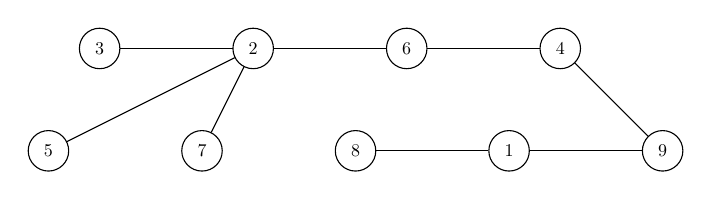
\begin{tikzpicture}[vertex/.style = {shape=circle,draw,minimum size=2.25em},scale=0.65, every node/.style={scale=0.65}]
    \node[vertex] (c1) at (-2,2) {$1$};
    \node[vertex] (c2) at (-7,4) {$2$};
    \node[vertex] (c3) at (-10,4) {$3$};
    \node[vertex] (c4) at (-1,4) {$4$};
    \node[vertex] (c5) at (-11,2) {$5$};
    \node[vertex] (c6) at (-4,4) {$6$};
    \node[vertex] (c7) at (-8,2) {$7$};
    \node[vertex] (c8) at (-5,2) {$8$};
    \node[vertex] (c9) at (1,2) {$9$};
    \draw (c1) -- (c9);
    \draw (c2) -- (c3);
    \draw (c2) -- (c5);
    \draw (c2) -- (c6);
    \draw (c2) -- (c7);
    \draw (c4) -- (c6);
    \draw (c1) -- (c8);
    \draw (c4) -- (c9);
\end{tikzpicture}
    \caption{The connections created by bijections for experimental class X.}
    \label{fig:expgrp_X}
\end{figure}


% experimental class 11
\begin{figure}[ht!]
    \centering
    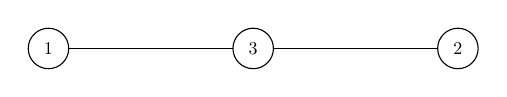
\begin{tikzpicture}[vertex/.style = {shape=circle,draw,minimum size=2.25em},scale=0.65, every node/.style={scale=0.65}]
    \node[vertex] (c1) at (0,0) {$1$};
    \node[vertex] (c2) at (8,0) {$2$};
    \node[vertex] (c3) at (4,0) {$3$};
    \draw (c2) -- (c3);
    \draw (c1) -- (c3);
\end{tikzpicture}
    \caption{The connections created by bijections for experimental class XI.}
    \label{fig:expgrp_XI}
\end{figure}


% experimental class 12 - Only 2 classes, no need to display
\begin{comment}
\begin{figure}[ht!]
    \centering
    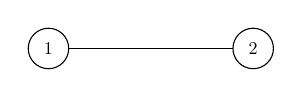
\begin{tikzpicture}[vertex/.style = {shape=circle,draw,minimum size=2.25em},scale=0.65, every node/.style={scale=0.65}]
    \node[vertex] (c1) at (0,0) {$1$};
    \node[vertex] (c2) at (4,0) {$2$};
    \draw (c1) -- (c2);
\end{tikzpicture}
    \caption{The connections created by bijections for experimental class XII.}
    \label{fig:expgrp_XII}
\end{figure}
\end{comment}


% experimental class 13
\begin{figure}[ht!]
    \centering
    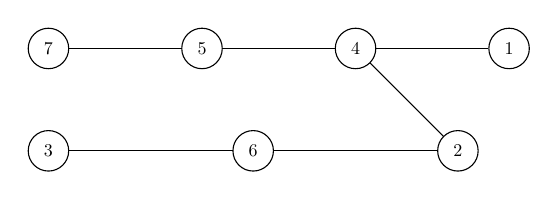
\begin{tikzpicture}[vertex/.style = {shape=circle,draw,minimum size=2.25em},scale=0.65, every node/.style={scale=0.65}]
    \node[vertex] (c1) at (3,0) {$1$};
    \node[vertex] (c2) at (2,-2) {$2$};
    \node[vertex] (c3) at (-6,-2) {$3$};
    \node[vertex] (c4) at (0,0) {$4$};
    \node[vertex] (c5) at (-3,0) {$5$};
    \node[vertex] (c6) at (-2,-2) {$6$};
    \node[vertex] (c7) at (-6,0) {$7$};
    \draw (c1) -- (c4);
    \draw (c2) -- (c6);
    \draw (c5) -- (c7);
    \draw (c2) -- (c4);
    \draw (c4) -- (c5);
    \draw (c3) -- (c6);
\end{tikzpicture}
    \caption{The connections created by bijections for experimental class XIII.}
    \label{fig:expgrp_XIII}
\end{figure}


% experimental class 14
\begin{figure}[ht!]
    \centering
    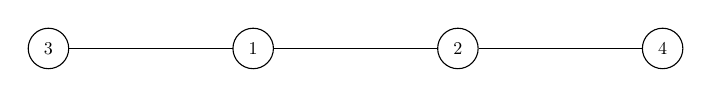
\begin{tikzpicture}[vertex/.style = {shape=circle,draw,minimum size=2.25em},scale=0.65, every node/.style={scale=0.65}]
    \node[vertex] (c1) at (-2,0) {$1$};
    \node[vertex] (c2) at (-6,0) {$3$};
    \node[vertex] (c3) at (2,0) {$2$};
    \node[vertex] (c4) at (6,0) {$4$};
    \draw (c1) -- (c2);
    \draw (c1) -- (c3);
    \draw (c3) -- (c4);
\end{tikzpicture}
    \caption{The connections created by bijections for experimental class XIV.}
    \label{fig:expgrp_XIV}
\end{figure}


% experimental class 15
\begin{figure}[ht!]
    \centering
    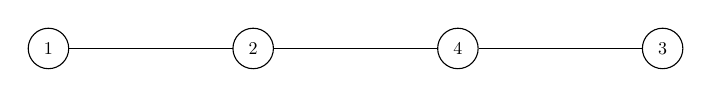
\begin{tikzpicture}[vertex/.style = {shape=circle,draw,minimum size=2.25em},scale=0.65, every node/.style={scale=0.65}]
    \node[vertex] (c1) at (-6,0) {$1$};
    \node[vertex] (c2) at (-2,0) {$2$};
    \node[vertex] (c3) at (6,0) {$3$};
    \node[vertex] (c4) at (2,0) {$4$};
    \draw (c1) -- (c2);
    \draw (c3) -- (c4);
    \draw (c2) -- (c4);
\end{tikzpicture}
    \caption{The connections created by bijections for experimental class XV.}
    \label{fig:expgrp_XV}
\end{figure}


% experimental class 16 - Only 2 classes, no need to display
\begin{comment}
\begin{figure}[ht!]
    \centering
    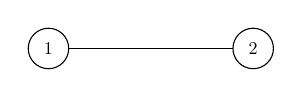
\begin{tikzpicture}[vertex/.style = {shape=circle,draw,minimum size=2.25em},scale=0.65, every node/.style={scale=0.65}]
    \node[vertex] (c1) at (0,0) {$1$};
    \node[vertex] (c2) at (4,0) {$2$};
    \draw (c1) -- (c2);
\end{tikzpicture}
    \caption{The connections created by bijections for experimental class XVI.}
    \label{fig:expgrp_XVI}
\end{figure}
\end{comment}


% experimental class 17
\begin{figure}[ht!]
    \centering
    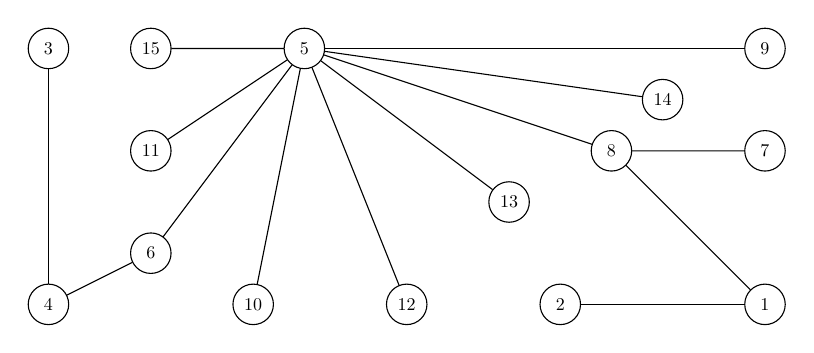
\begin{tikzpicture}[vertex/.style = {shape=circle,draw,minimum size=2.25em},scale=0.65, every node/.style={scale=0.65}]
    \node[vertex] (c1) at (7,0) {$1$};
    \node[vertex] (c2) at (3,0) {$2$};
    \node[vertex] (c3) at (-7,5) {$3$};
    \node[vertex] (c4) at (-7,0) {$4$};
    \node[vertex] (c5) at (-2,5) {$5$};
    \node[vertex] (c6) at (-5,1) {$6$};
    \node[vertex] (c7) at (7,3) {$7$};
    \node[vertex] (c8) at (4,3) {$8$};
    \node[vertex] (c9) at (7,5) {$9$};
    \node[vertex] (c10) at (-3,0) {$10$};
    \node[vertex] (c11) at (-5,3) {$11$};
    \node[vertex] (c12) at (0,0) {$12$};
    \node[vertex] (c13) at (2,2) {$13$};
    \node[vertex] (c14) at (5,4) {$14$};
    \node[vertex] (c15) at (-5,5) {$15$};
    \draw (c1) -- (c2);
    \draw (c3) -- (c4);
    \draw (c5) -- (c6);
    \draw (c7) -- (c8);
    \draw (c4) -- (c6);
    \draw (c1) -- (c8);
    \draw (c5) -- (c8);
    \draw (c5) -- (c9);
    \draw (c5) -- (c10);
    \draw (c5) -- (c11);
    \draw (c5) -- (c12);
    \draw (c5) -- (c13);
    \draw (c5) -- (c14);
    \draw (c5) -- (c15);
\end{tikzpicture}
    \caption{The connections created by bijections for experimental class XVII.}
    \label{fig:expgrp_XVII}
\end{figure}


% experimental class 18
\begin{figure}[ht!]
    \centering
    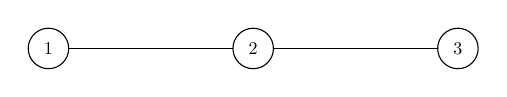
\begin{tikzpicture}[vertex/.style = {shape=circle,draw,minimum size=2.25em},scale=0.65, every node/.style={scale=0.65}]
    \node[vertex] (c1) at (0,0) {$1$};
    \node[vertex] (c2) at (4,0) {$2$};
    \node[vertex] (c3) at (8,0) {$3$};
    \draw (c2) -- (c3);
    \draw (c1) -- (c2);
\end{tikzpicture}
    \caption{The connections created by bijections for experimental class XVIII.}
    \label{fig:expgrp_XVIII}
\end{figure}


% experimental class 19
\begin{figure}[ht!]
    \centering
    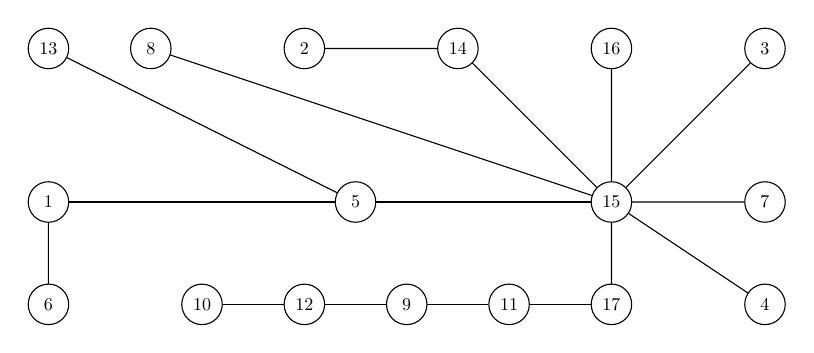
\begin{tikzpicture}[vertex/.style = {shape=circle,draw,minimum size=2.25em},scale=0.65, every node/.style={scale=0.65}]
    \node[vertex] (c1) at (-8,3) {$1$};
    \node[vertex] (c2) at (-3,6) {$2$};
    \node[vertex] (c3) at (6,6) {$3$};
    \node[vertex] (c4) at (6,1) {$4$};
    \node[vertex] (c5) at (-2,3) {$5$};
    \node[vertex] (c6) at (-8,1) {$6$};
    \node[vertex] (c7) at (6,3) {$7$};
    \node[vertex] (c8) at (-6,6) {$8$};
    \node[vertex] (c9) at (-1,1) {$9$};
    \node[vertex] (c10) at (-5,1) {$10$};
    \node[vertex] (c11) at (1,1) {$11$};
    \node[vertex] (c12) at (-3,1) {$12$};
    \node[vertex] (c13) at (-8,6) {$13$};
    \node[vertex] (c14) at (0,6) {$14$};
    \node[vertex] (c15) at (3,3) {$15$};
    \node[vertex] (c16) at (3,6) {$16$};
    \node[vertex] (c17) at (3,1) {$17$};
    \draw (c10) -- (c12);
    \draw (c3) -- (c15);
    \draw (c11) -- (c17);
    \draw (c5) -- (c13);
    \draw (c2) -- (c14);
    \draw (c5) -- (c15);
    \draw (c9) -- (c11);
    \draw (c8) -- (c15);
    \draw (c9) -- (c12);
    \draw (c15) -- (c17);
    \draw (c7) -- (c15);
    \draw (c6) -- (c1);
    \draw (c4) -- (c15);
    \draw (c14) -- (c15);
    \draw (c15) -- (c16);
    \draw (c1) -- (c5);
\end{tikzpicture}
    \caption{The connections created by bijections for experimental class XIX.}
    \label{fig:expgrp_XIX}
\end{figure}


% experimental class 20
\begin{figure}[ht!]
    \centering
    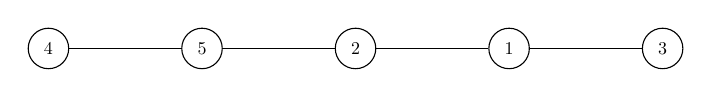
\begin{tikzpicture}[vertex/.style = {shape=circle,draw,minimum size=2.25em},scale=0.65, every node/.style={scale=0.65}]
    \node[vertex] (c1) at (0,0) {$1$};
    \node[vertex] (c2) at (-3,0) {$2$};
    \node[vertex] (c3) at (3,0) {$3$};
    \node[vertex] (c4) at (-9,0) {$4$};
    \node[vertex] (c5) at (-6,0) {$5$};
    \draw (c1) -- (c2);
    \draw (c1) -- (c3);
    \draw (c4) -- (c5);
    \draw (c2) -- (c5);
\end{tikzpicture}
    \caption{The connections created by bijections for experimental class XX.}
    \label{fig:expgrp_XX}
\end{figure}

% experimental class 21
\begin{figure}[ht!]
    \centering
    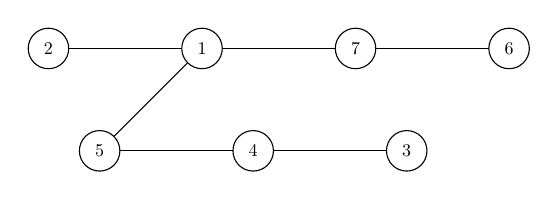
\begin{tikzpicture}[vertex/.style = {shape=circle,draw,minimum size=2.25em},scale=0.65, every node/.style={scale=0.65}]
    \node[vertex] (c1) at (0,2) {$1$};
    \node[vertex] (c2) at (-3,2) {$2$};
    \node[vertex] (c3) at (4,0) {$3$};
    \node[vertex] (c4) at (1,0) {$4$};
    \node[vertex] (c5) at (-2,0) {$5$};
    \node[vertex] (c6) at (6,2) {$6$};
    \node[vertex] (c7) at (3,2) {$7$};
    \draw (c1) -- (c2);
    \draw (c3) -- (c4);
    \draw (c4) -- (c5);
    \draw (c6) -- (c7);
    \draw (c1) -- (c7);
    \draw (c1) -- (c5);
\end{tikzpicture}
    \caption{The connections created by bijections for experimental class XXI.}
    \label{fig:expgrp_XXI}
\end{figure}


% experimental class 22
\begin{figure}[ht!]
    \centering
    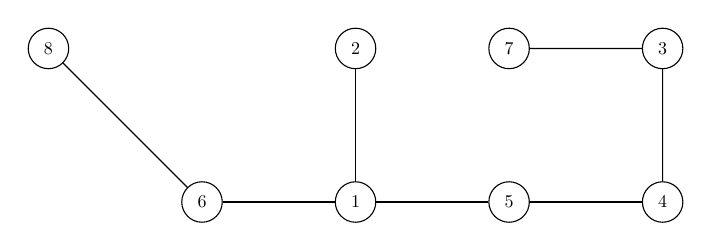
\begin{tikzpicture}[vertex/.style = {shape=circle,draw,minimum size=2.25em},scale=0.65, every node/.style={scale=0.65}]
    \node[vertex] (c1) at (0,0) {$1$};
    \node[vertex] (c2) at (0,3) {$2$};
    \node[vertex] (c3) at (6,3) {$3$};
    \node[vertex] (c4) at (6,0) {$4$};
    \node[vertex] (c5) at (3,0) {$5$};
    \node[vertex] (c6) at (-3,0) {$6$};
    \node[vertex] (c7) at (3,3) {$7$};
    \node[vertex] (c8) at (-6,3) {$8$};
    \draw (c4) -- (c5);
    \draw (c1) -- (c5);
    \draw (c3) -- (c4);
    \draw (c6) -- (c8);
    \draw (c7) -- (c3);
    \draw (c6) -- (c1);
    \draw (c2) -- (c1);
\end{tikzpicture}
    \caption{The connections created by bijections for experimental class XXII.}
    \label{fig:expgrp_XXII}
\end{figure}


% experimental class 23
\begin{figure}[ht!]
    \centering
    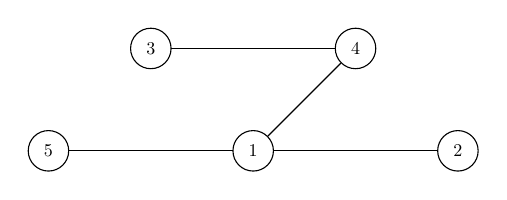
\begin{tikzpicture}[vertex/.style = {shape=circle,draw,minimum size=2.25em},scale=0.65, every node/.style={scale=0.65}]
    \node[vertex] (c1) at (0,0) {$1$};
    \node[vertex] (c2) at (4,0) {$2$};
    \node[vertex] (c3) at (-2,2) {$3$};
    \node[vertex] (c4) at (2,2) {$4$};
    \node[vertex] (c5) at (-4,0) {$5$};
    \draw (c1) -- (c2);
    \draw (c3) -- (c4);
    \draw (c1) -- (c4);
    \draw (c1) -- (c5);
\end{tikzpicture}
    \caption{The connections created by bijections for experimental class XXIII.}
    \label{fig:expgrp_XXIII}
\end{figure}


% experimental class 24 - Only 2 classes, no need to display
\begin{comment}
\begin{figure}[ht!]
    \centering
    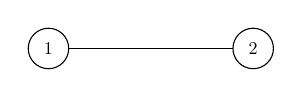
\begin{tikzpicture}[vertex/.style = {shape=circle,draw,minimum size=2.25em},scale=0.65, every node/.style={scale=0.65}]
    \node[vertex] (c1) at (0,0) {$1$};
    \node[vertex] (c2) at (4,0) {$2$};
    \draw (c2) -- (c1);
\end{tikzpicture}
    \caption{The connections created by bijections for experimental class XXIV.}
    \label{fig:expgrp_XXIV}
\end{figure}
\end{comment}


% experimental class 25 - Only 2 classes, no need to display
\begin{comment}
\begin{figure}[ht!]
    \centering
    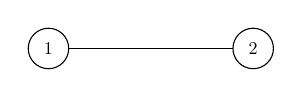
\begin{tikzpicture}[vertex/.style = {shape=circle,draw,minimum size=2.25em},scale=0.65, every node/.style={scale=0.65}]
    \node[vertex] (c1) at (0,0) {$1$};
    \node[vertex] (c2) at (4,0) {$2$};
    \draw (c1) -- (c2);
\end{tikzpicture}
    \caption{The connections created by bijections for experimental class XXV.}
    \label{fig:expgrp_XXV}
\end{figure}
\end{comment}


% experimental class 26
\begin{figure}[ht!]
    \centering
    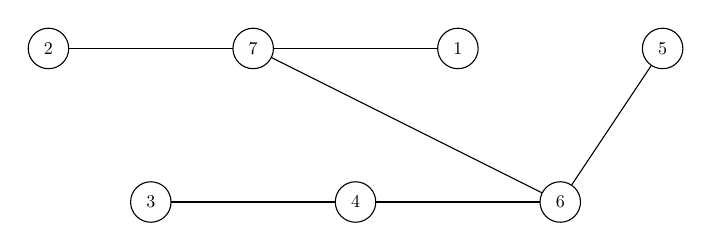
\begin{tikzpicture}[vertex/.style = {shape=circle,draw,minimum size=2.25em},scale=0.65, every node/.style={scale=0.65}]
    \node[vertex] (c1) at (0,3) {$1$};
    \node[vertex] (c2) at (-8,3) {$2$};
    \node[vertex] (c3) at (-6,0) {$3$};
    \node[vertex] (c4) at (-2,0) {$4$};
    \node[vertex] (c5) at (4,3) {$5$};
    \node[vertex] (c6) at (2,0) {$6$};
    \node[vertex] (c7) at (-4,3) {$7$};
    \draw (c6) -- (c7);
    \draw (c5) -- (c6);
    \draw (c4) -- (c6);
    \draw (c3) -- (c4);
    \draw (c2) -- (c7);
    \draw (c1) -- (c7);
\end{tikzpicture}
    \caption{The connections created by bijections for experimental class XXVI.}
    \label{fig:expgrp_XXVI}
\end{figure}